%% Fjalar design document
\documentclass[11pt]{article}
\usepackage[pdftex]{graphicx} 
\usepackage{listings}
\usepackage{program}
\usepackage{wrapfig}
\title{Implementation of Fjalar}
\date{}
\author{}
\begin{document} \maketitle
This chapter outlines the implementation of Fjalar, a dynamic analysis
framework for C/C++ programs. 

Fjalar can be broken down into 3 primary modules: The DWARF parser,
which transforms the DWARF information in a program
binary into a more suitable representation, the function
instrument, which inserts calls into Fjalar at function entries and
exits of a target program, and the variable traverser, which
collects information about program variables. A diagram of these 3
modules, including their inputs is provided below.

\begin{figure}
\noindent
\centering
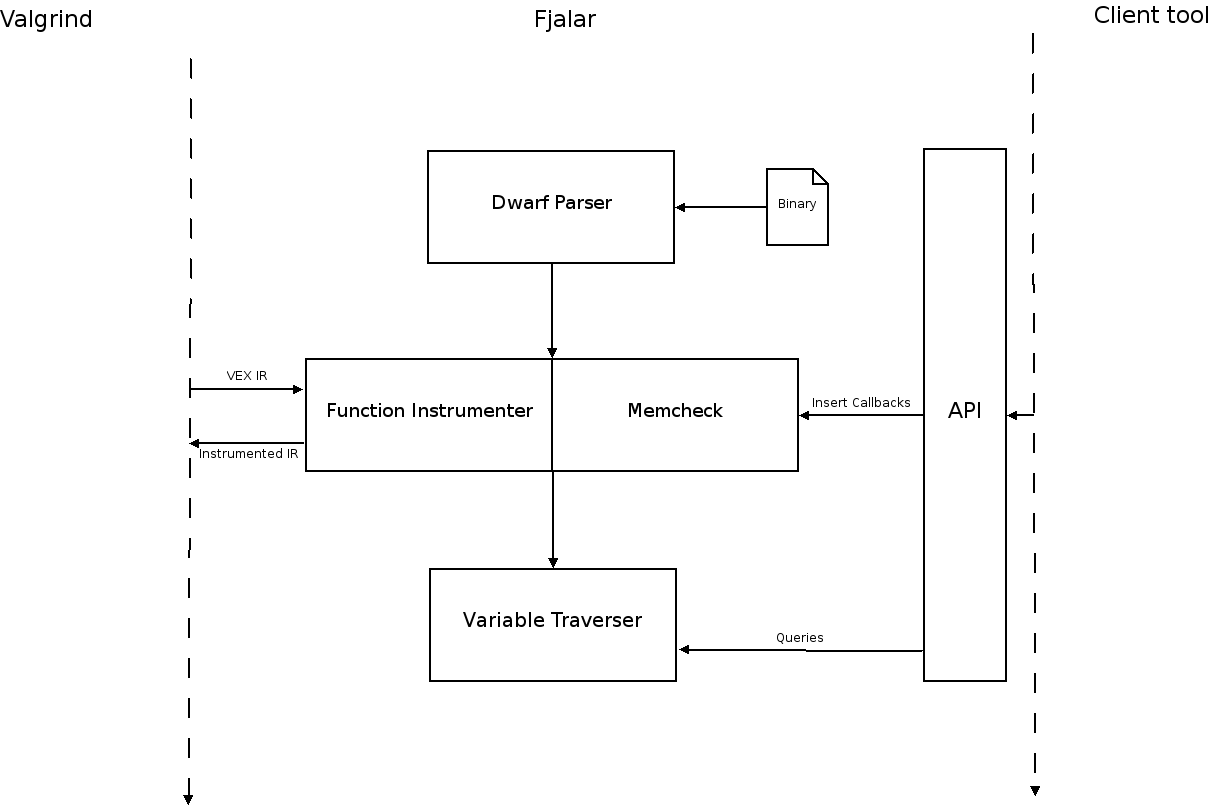
\includegraphics[width=150mm]{fjalar-arch-initial.png}
\caption{Fjalar architecture}
\end{figure}

This chapter is organized into the following sections: 

\begin{itemize}
\item Section 1 describes Fjalar's DWARF parser
\item Section 2 describes Fjalar's Function instrumenter
\item Section 3 describes Fjalar's Variable traverser
\item Section 4 details Fjalar's API as well as provides an
  implementation of a simple tool
\end{itemize}

\section{The DWARF Parser}
\subsection{The DWARF debugging format}
The purpose of debugging information is to provide a mapping between
the low-level information contained in a binary and the symbolic,
high-level constructs present in the source code. This mapping is
designed to allow debuggers to present higher level and more useful
information to a programmer than it could otherwise.

DWARF is a standardized format for debugging information
\cite{silverstein1993dwarf}. There are currently 3 versions of the
DWARF format. DWARF version 1 was developed and released in the mid
1980s, but never achieved widespread use due to inefficiencies. DWARF
version 2 was released in 1990 and is currently the standard debugging
format used by Linux binaries. Fjalar is only designed to work with
DWARF version 2. DWARF version 3 was released in 2006 and has yet to
gain wide-use, though it is backwards compatible with DWARF version 2.

Fjalar leverages the information available in the DWARF format to
provide an interface for tools to read and modify data in a target
program using source-level constructs.

%**NOTE**: Should I go into depth on the DWARF format

\subsection{Readelf hooks}
Due to the complex nature of both the DWARF debugging information and
the ELF binary format (the standard object file format on Linux),
Fjalar makes use of readelf, a component of GNU Binutils designed to
display information on ELF object files. Fjalar contains a modified
version of readelf in which all the functions for displaying DWARF
information contain callbacks into Fjalar. \texttt{typedata.c} is
responsible for constructing a very low-level, but organized version
of the DWARF information. This low-level representation closely mimics
the internal structure of the DWARF information, but is not an
appropriate representation for the work Fjalar must do.

\subsection{Translating DWARF information into Fjalar data structures}
The majority of Fjalar's compile-time information is represented by
three data structures: (1) FunctionEntry, (2) VariableEntry, and (3)
TypeEntry. Their declarations can be located in \texttt{fjalar\_include.h}

\subsubsection{FunctionEntry}
The FunctionEntry structure contains information about a particular
function. It contains the function's name, the name of the file in which  
the function is defined, the start and end address of the function's 
instructions, whether or not the function is declared as file-static,
and lists of the function's formal parameters and local variables. 

When dealing with C++ programs, a function's FunctionEntry will also  
contain the mangled and demangled name of the function and, if it's a
member function, a pointer to the TypeEntry of its enclosing class.

\subsubsection{VariableEntry}
The VariableEntry structure contains information about a particular
variable in the program. It contains the name of the variable, whether
it is a global, local, formal parameter, or return variable, the
location of the variable and itss declared type. Additionally,
if it is a member variable it contains a pointer to its enclosing
class, struct, or union.

\subsubsection{TypeEntry}
The TypeEntry structure contains information about a particular type used
by the program. There are premade type entries for all the primitive
types defined in C and C++, such as char, int, long, etc.A TypeEntry
contains  the
declared type of the variable, the name of the type, and the size of
the type in bytes.

If the type corresponds to a struct, class, or union (this is referred to
as an aggregate type throughout the Fjalar codebase), it contains a pointer
to an AggregateType structure which contains additional information
including a list of all member variables and, in the case of C++
classes, a list of constructors, destructors, and superclasses.

\subsubsection{Translation}
\texttt{generate\_fjalar\_entries.c} is responsible for translating the low-level
representation provided by \texttt{typedata.c} and translating it into the above
Fjalar data structures. It accomplishes this by taking the representation of
the DWARF data and making 2 passes across it. First it makes a pass
for functions. During this pass Fjalar creates a FunctionEntry for every function contained
in the debugging information and creates 2 hash tables for accessing
them. One hash table is indexed by the address of the function's starting
address (referred to as the startPC), the second is indexed by the
address of the instruction corresponding to the first line of code
(referred to as the entryPC). 

It then makes a second pass over the representation, creating  a 
VariableEntry and, if necessary, a TypeEntry for every Variable. It is
at this point that it associates formal parameters and local variables
with their containing functions, as well as creating a list of all the
global variables in the program.

Finally the function table is iterated over once to make sure that
member functions and constructors/destructors are correctly referenced
by their enclosing class's TypeEntry.

This entire process takes linear time proportional to the size of the
debugging information. This process finishes fairly fast for most
programs, even particularly large C programs. Large C++ programs,
particularly those which make use of templates, are known to contain
large amounts of debugging information \cite{rotithor1999measurement}
and as such will take longer to process.

\section{Function entry and exit handling}
Fjalar instruments the entry and exit of every function in the target
program. This instrumentation is to allow Fjalar to collect any
information necessary to perform a variable traversal of the function
(detailed in the following section) and to run any code requested by
the client tool.


\subsection{Determining entries and exits}
The DWARF information provides the first instruction and last
instructions of a function. Unfortunately, this
is insufficient for detecting entries and exits for a few reasons:

For entries, we would prefer to enter after the prologue of the
function has run, as the variable information provided by the DWARF
information tends to be valid for a function with a valid stack frame.
Fjalar

For exits, the last instruction only corresponds to one possible
exit. However, for functions with multiple exit points, the compiler
may choose to have multiple instructions which exit the function, so
going by the last instruction is not enough. Luckily, Valgrind
translates all exits out of a function into a special IR which makes
Fjalar's job easier

Valgrind allows any tool built upon it to instrument every basic block
of VEX IR before it performs the final translation back. For every
basic block Fjalar performs the following algorithm to find VEX
instructions which correspond to a function entry:

\begin{program}
For every Function f:
  f.entryPC = f.firstline in DWARF[f];

iMax = 0
For every IMark instruction i:
  Look up i in FunctionEntryByStartPC 
  if functionEntry f is found:
    iMax = i
    For the remaining instructions j in i's basic block
      if j <= f.entryPC: 
        iMax = j
if iMax != 0:
  Insert enter\_function(f) before iMax

Determining exits is easier due to the VEX Instruction type
Ist\_Exit. To determine exits:
o
For every Exit instruction i:
  For every function f:
     if f.startPC < i and f.endPC > i:
        insert exit\_function(f) before i
\end{program}

\subsubsection{Non-local exits}
Non-local exits are particularly troublesome for Fjalar due to the
fact that they do will not show up as a normal function exit in the
assembly, and accordingly do not show up in the VEX IR as EXIT
instructions. Because of this Fjalar will currently not execute exit
instrumentation for any functions that were non-locally exited.

\section{Variable Traversal}
Due to the memory-unsafe nature of C/C++ safely exploring the
variables in a target C/C++ program is a difficult
proposition. Accordingly, the handling of variable traversal is the
complex aspect of Fjalar. Variables can be broken into 2 groups:
normal variables % This is a terrible name, think of a better name % 
and pointers and arrays

For both cases the DWARF information provides us with enough
information to locate the beginning of the variable.

\subsection{Translating DWARF locations}
Locations in the DWARF information are provided as a sequence of
DWARF expressions. Each DWARF expression is itself made up of a DWARF
operator and one or more DWARF atoms. All DWARF expressions work. In
addition to the DWARF atoms the DWARF operations may also perform
operations on an implicit stack. The DWARF location information can be
thought of as an instruction set for a very simple stack machine.

Fjalar currently implements a subset of this instruction set. Fjalar's
interpreter can be found in fjalar\_traversal.c and complete
information about the set of DWARF operations can be find in
include/elf/dwarf2.h and the DWARF website %link

\subsection{Normal Variables} % change name
For these variables, Fjalar simply executes the sequence of DWARF
expressions in the DWARF information to determine the variable's
address in memory. Variables contained in registers do not need to be treated
specially as Valgrind keeps an in-memory structure of the target
program's register state. This memory address is returned to the
client tool

\subsection{Pointers and Arrays}
Pointer and array variables give Fjalar the most trouble. The C
language standard does not require that pointers point to a valid
location at all points in the program. Instead it leaves the behavior
of dereferencing pointers which point to invalid locations, such as
NULL or a location that was recently free()'d among others, as
undefined. This makes Fjalar's job of performing variable traversal
hard. Due to the duality of pointers and arrays in C/C++, the above
also applies to arrays.

Fjalar aims to provide a way to access all non-local variables 
in scope at a given function entry or exit. For all in-scope variable
Fjalar provides information about the variables such as its type,
its name, levels of pointer indirection, and the address of the
variable in memory. Fjalar is able to provide the exact location in
memory due to running in the same memory space as the target
program. The VALGRIND PAPER %TODO find and reference% 
describes in detail the subtleties involved in achieving this
robustly.

%% The below needs to be restructured. As with C Fjalar doesn't really
%% handle arrays and pointers in a separate manner. Pointers are just
%% consider to point to many possible elements, if it points > 1
%% elements it's a ``sequence'' (fjalar's term for arrays)

\subsubsection{Pointers}
In addition to the variable information mentioned in the previous
section, Fjalar would like to recursively provide the
address in memory of any pointed to variables. For example In the
following code segment:

int *ptr1;
int **ptr2;

Fjalar would like to provide the address of *ptr1, ptr1, **ptr2,
*ptr2, and ptr2. The ptr1 case is relatively trivial because if ptr1
was a propelry declared variable, The compiler will have allocated
space somewhere in the program's memory/register space for the
variable (This assumption does not hold in the case of optimized
programs, which Fjalar does not currently support). So in the case of
ptr1 it's simply an issue of providing the address of *ptr, and the
value at that address.

ptr2, however, is much more problematic. **ptr2 and *ptr2 are easy for
the same reasons mentioned above. Providing the address of ptr2,
however, requires Fjalar to examine a memory location provided by the
easier. It's worthwhile to ensure the subtle differnce between the
difficulty in these 2 cases.The address of **ptr2 is most likely safe
to dereference as it's an automatic variable and has been propelrly
allocated by the compiler, thus finding the address of *ptr2 is easy,
it just requires reading the value at the address of **ptr2. the value
in **ptr2 may be garbage or program, however we do not need to actually
dereference this value to provide the address of *ptr2.

Providing the address of ptr2, however, does require to dereference
this value. This is a very unsafe operation, and could cause both
Fjalar and the target program to crash if the address we use is
invalid. This is obviously unacceptable. To counteract this Fjalar
makes use of Memcheck to ensure this operation is safe. Fjalar queries
Memcheck before accessing any memory location in the target
program, If Memcheck reports the address as either unallocated or
uninitialized Fjalar will not due the dereference and simply mark the
variable as such before passing it to the tool

\subsubsection{Arrays}
The DWARF information gives us some aid in regards to determining the
length of an array. The DWARF information provides us with
size information for arrays allocated on the stack or in global
memory.

This makes it trivial to provide the size for a global array, arrays
passed as a function argument, however, are more difficult. C does not
support passing an array by value, so when passed to a function,
arrays are decayed into a pointer. To determine whether or not a
pointer argument is an array Fjalar employs the following algorithm to
determine the length of the array.



1. Determine If the address points to the global address space, if so
   try and find a global variable in the DWARF information that could
   correspond to this address. This involves both an equality comparison
   between the address of all variables in the global space, and checking
   if this address is in the bounds of another array.
   
   If a corresponding variable is found, this is a pointer. If this lies
   between the bounds of a global array, this is an array of size
   (global\_arr\_end\_addr - addr). Continue to step 2 if no
   corresponding variable found.

2. Determing if the address points to a array currently on the stack,
   To do this, Fjalar iterates over all functions currently on the
   stack to try and find one in it's stack frame, Fjalar determines a
   the address range of function's stack frame by subtracting the
   stored stack pointer from the stored frame pointer. If it is in
   some function's stack space, it searches all of the function's
   local variables for a corresponding vaariable with a search
   identical to the 1 proposed in 1

3. This step is broken into 2 cases:

   address in the stack or global region, but no corresponding
   variable found in previous searches: return size of 1.

   All other variables:
   
   Continously query memcheck for every address from the initial
   address onwards. Return a size of (last\_initialized\_address -
   initial address).


The first two methods provide relatively accurate results. The 3rd
method is used as a last resort in the case of heap allocations, or
addresses in the stack which have no corresponding variable. This
tends to grossly estimate array size, as depending on the allocation
tendencies of the target program, the entire length of a dynamically
allocated block does not always correspond to the length of a single
array in the program.


\section{Fjalar API}

This section goes over the primary functions of the Fjalar API. Every
tool must implement the following 2 functions:

\subsection{Function instrumentation}

void fjalar\_tool\_handle\_function\_entrance(FunctionExecutionState* f\_state);
void fjalar\_tool\_handle\_function\_exit(FunctionExecutionState*
f\_state);

Fjalar will call insert a call to the first function after the
prologue of every function in the target program. It will insert a
call to the second instruction before the RET instruction of every
function in the target program. The FunctionExecutionState will
contain some of the dynamic state of the instrumented function at the
time of the call, including the address of the top of the stack, the
beginning of the current stack frame, A complete copy of all the
values on the function's stack at entry (this is done to allow
analysis of formal parameters even in situatoins where the compiler
chooses to use their locations on the stack to store temporaries). 
Additionally it contains a pointer to a FunctionEntry struct which
contains the sum of static information known about the function, this
was discussed in detail in section %TODO x.1.3.1

Consider the code fragment below:

\lstset{language=C, frame=single}
\begin{lstlisting}
int main(int argc, char **argv) {
  int b = 5;
  int *p = &b, *q;
  return 5;
}
\end{lstlisting}

Fjalar will instrument the code and insert a call before before the
first instruction of the 'int b = 5', and one more before the last
instruction of the 'return 5'. An example of the pre and post
instrumented  VEX IR is included below

%%TODO INCLUDE EXAMPLE

\subsection{Variable Inspection}

Fjalar allows a client tool to inspect all non-local  variables in
scope at a given function entry or exit. This is done through the
function 

void visitVariableGroup

The tooler provides the variable group to traverse (either global
variables, formal parameters, or the return value) and a callback
function. Fjalar will then call the callback for every variable within
the group, providing it with a VariableEntry as well as auxiliary
information such as it's location in memory, whether or not it's a
sequence of elements, and the number of elements.) Additionally,
Fjalar provides a few convenience functions to examine individual
variables given a VariableEntry, however the information provided is
much more limited as it is unable to determine things like memory
location and number of elements without the run-time information
provided by a functionExecutionState.

Below is an example client  which makes use of the Fjalar API to print
the memory location of all variables

\bibliographystyle{plain}
\bibliography{fjalar}
\end{document}



